\chapter{Methodology}
\label{chapterlabel3}

This study analyses the performance exhibited by the Deep Gravity and Production-constrained models concerning work-related and non-work-related flows within London. As a result, this work establishes a comprehensive comparison between the outcomes generated by these models and the observed flow patterns present in the context of London. This comparative investigation provides a more robust understanding of the efficacy and applicability of the Deep Gravity and Production-constrained models.



% STUDY AREA

    \section{Study Area}

This study focuses on the entire region of London,  its inner and outer areas. London has diverse cultures, nationalities, incomes, transportation options, public services, and amenities. To truly understand how people travel across the city, looking at the entire region is essential. This approach intends to understand the commuting patterns, considering all the factors contributing to how people move around in this diverse and dynamic urban environment.


%%% DATA

    \section{Data}

This study relies on three primary datasets: Locomizer, Point of Interest, and Census 2021. Locomizer serves as the central component of the analysis, with the aggregated origin and destination flow for London within hexagons as geographic area units. The hexagon ID serves as the primary index, and to ensure coherence, the remaining datasets are incorporated into this index via an area-weighted spatial join.

    \begin{figure}[H]
        \centering
        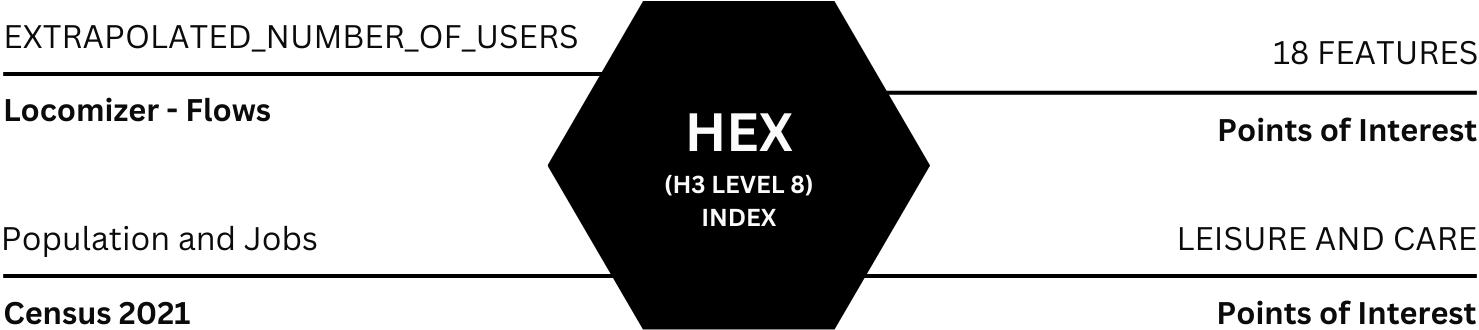
\includegraphics[width=12cm]{Images/framework.png}
        \caption{Methodology framework}
        \label{fig: framework}
    \end{figure}


%%% Mobility Data
     \subsection{Mobility data} 

The Locomizer is a  human mobility dataset derived from mobile phone devices, ensuring that the participants have explicitly consented to utilise their data. This dataset contains a variety of key metrics. It captures observed and extrapolated counts of users who have spent time within a specified geographic area over a specific timeframe. Moreover, it includes the number of signals, effectively representing observations, at each location.

These metrics are organised based on different movement categories, distinguishing between pedestrian and non-pedestrian activities. Additionally, the dataset categorises users based on visitation modalities,  differentiating "workers" from the overall population. Identifying the "common daytime location (CDL)" or the workplace for these worker users is accomplished by analysing device-level data and areas with the highest dwell time during typical working hours. This specific analysis aids in understanding and inferring the work-related locations of these users. To decrease granularity, worker users are aggregated, and the resulting data is presented at the point level, utilising a 69-meter radius around each point of interest (POI).

The dataset applied in this study contains aggregated data at level 9(Figure \ref{fig: grid 7}, with each dataset file including more than 4 million rows. The careful cleaning of this dataset emerged as an essential requirement to ensure the integrity of subsequent analyses. Hexagons play a key role in understanding spatial relationships, particularly mobility flows. Despite the computational limitation of running the spatial interaction model to deal with a high amount of data,  it required a transition from hexagonal level 9 to level 7. This transformation was facilitated through the H3 package\citep{uberTablesCellStatistics2023} in Python. At level 9, a hexagon has a relatively small area, approximately 0.10 square kilometres. In contrast, at level 7, a hexagon covers a significantly larger area, approximately 5.16 square kilometres.

    \begin{figure}[H]
        \centering
        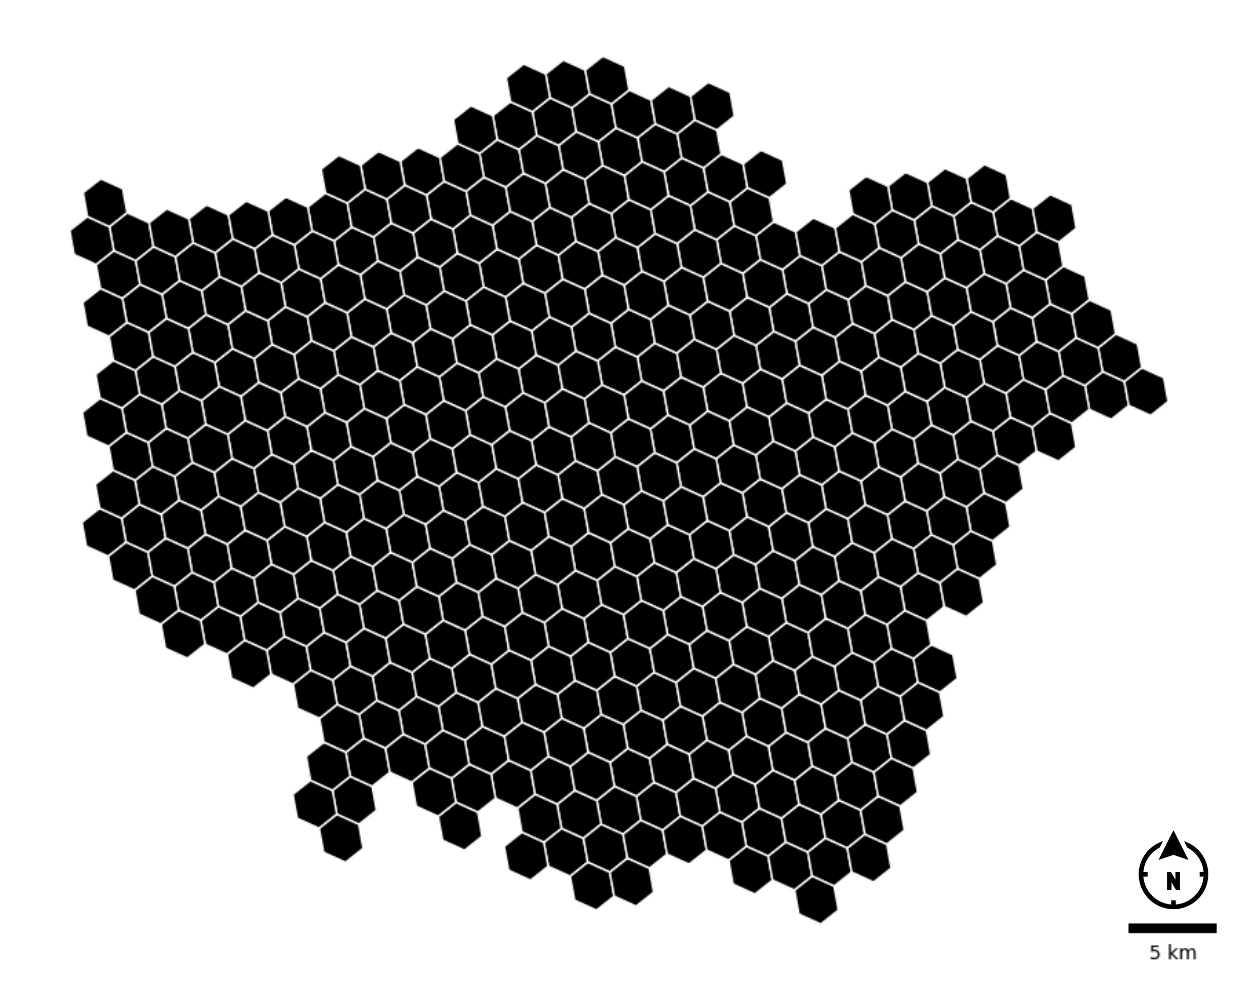
\includegraphics[width=10cm]{Images/Hexagons_level7.png}
        \caption{London in Hexagons at level 7}
        \label{fig: grid 7}
    \end{figure}  
    
The dataset contains two fundamental segments: the origins, while the other relates to destinations. Both datasets are characterised by columns ORIGIN and DESTINATION. However, only the top 100 destinations were retained within the' Origin' segment. On the other hand, only the top 100 origins were incorporated in the' Destination' segment. This approach provides a more comprehensive overview of the system's dynamics. Flows lacking a defined origin or destination, denoted by '0' entries, were excluded. Moreover, it eliminated duplicated flow instances from the final dataset.

The 'extrapolated number of users' concept is introduced to estimate user presence within a specific geographic region over a designated time frame. Diverse movement modalities are available in the dataset, with the entirety ('all') and the workforce ('workers'). The 'transient' aspect, defined as the difference between the overall movement and the workforce, is established for non-work flows. The dataset explores variations in movement modes, such as walking/non-walking. However, this study considers the 'All' categorization to investigate the general mobility patterns.

It was chosen to focus only on data from a single day despite the availability of extensive datasets. Wednesday was chosen as the focus day to represent a regular workday without exceptional events, such as strikes. Additionally, Sunday was considered suitable for examining non-work-related movements, providing insights into mobility unaffected by work duties.

The Table \ref{table: Locomizer features} below summarizes the main aspects of the dataset. It provides insights into the utilized hexagonal grid, the identifiers for origin and destination points, the mode of movement, the temporal scope of analysis, and the specific days selected for work-related and non-work-related flows.





\begin{table}[H]
\centering
\begin{tabular}{ll}
\hline
\textbf{Features}   & \textbf{Description}        \\ \hline
\textbf{Grid}               & Uber H3 hexagons at Level 8 \\
\textbf{Origin\_Code}        & Origin HEX ID               \\
\textbf{Destination\_Code}   & Destination HEX ID          \\
\textbf{Visitation Modality} & All                         \\
\textbf{Movement Modality}   & All/ Workers/ Transients¹   \\
\textbf{Daytime}             & 25 (00.00-23.59)            \\ 
\textbf{Work Flow Date}      & 08/03/2023 (Wednesday)      \\ 
\textbf{Non-work Flow Date}  & 12/03/2023 (Sunday)         \\ \bottomrule
\end{tabular}
    \caption{Features classification - Locomizer Dataset}
    \label{table: Locomizer features}
\end{table}

Hexagons at level 7 in London have 415 hexagons, resulting in 172,225 possible origin and destination flow combinations. Consequently, the dataset concerning work and workflows displays a distinct distribution, as shown in Figure \ref{fig: Data Values Overview}. This distinction arises because workflows constitute only a fraction of the overall flow. As a result, this dataset showcases both a reduced maximum value and a lower mean value. This value difference leads to a more balanced workflow data distribution, as the accompanying graph shows. Furthermore, the distance from the mean (standard deviation) is notably smaller. Therefore, the values shown in the graphs are presented in logarithmic scale to accommodate the dataset's extensive size and prevent value distortion.


    \begin{figure}[H]
        \centering
        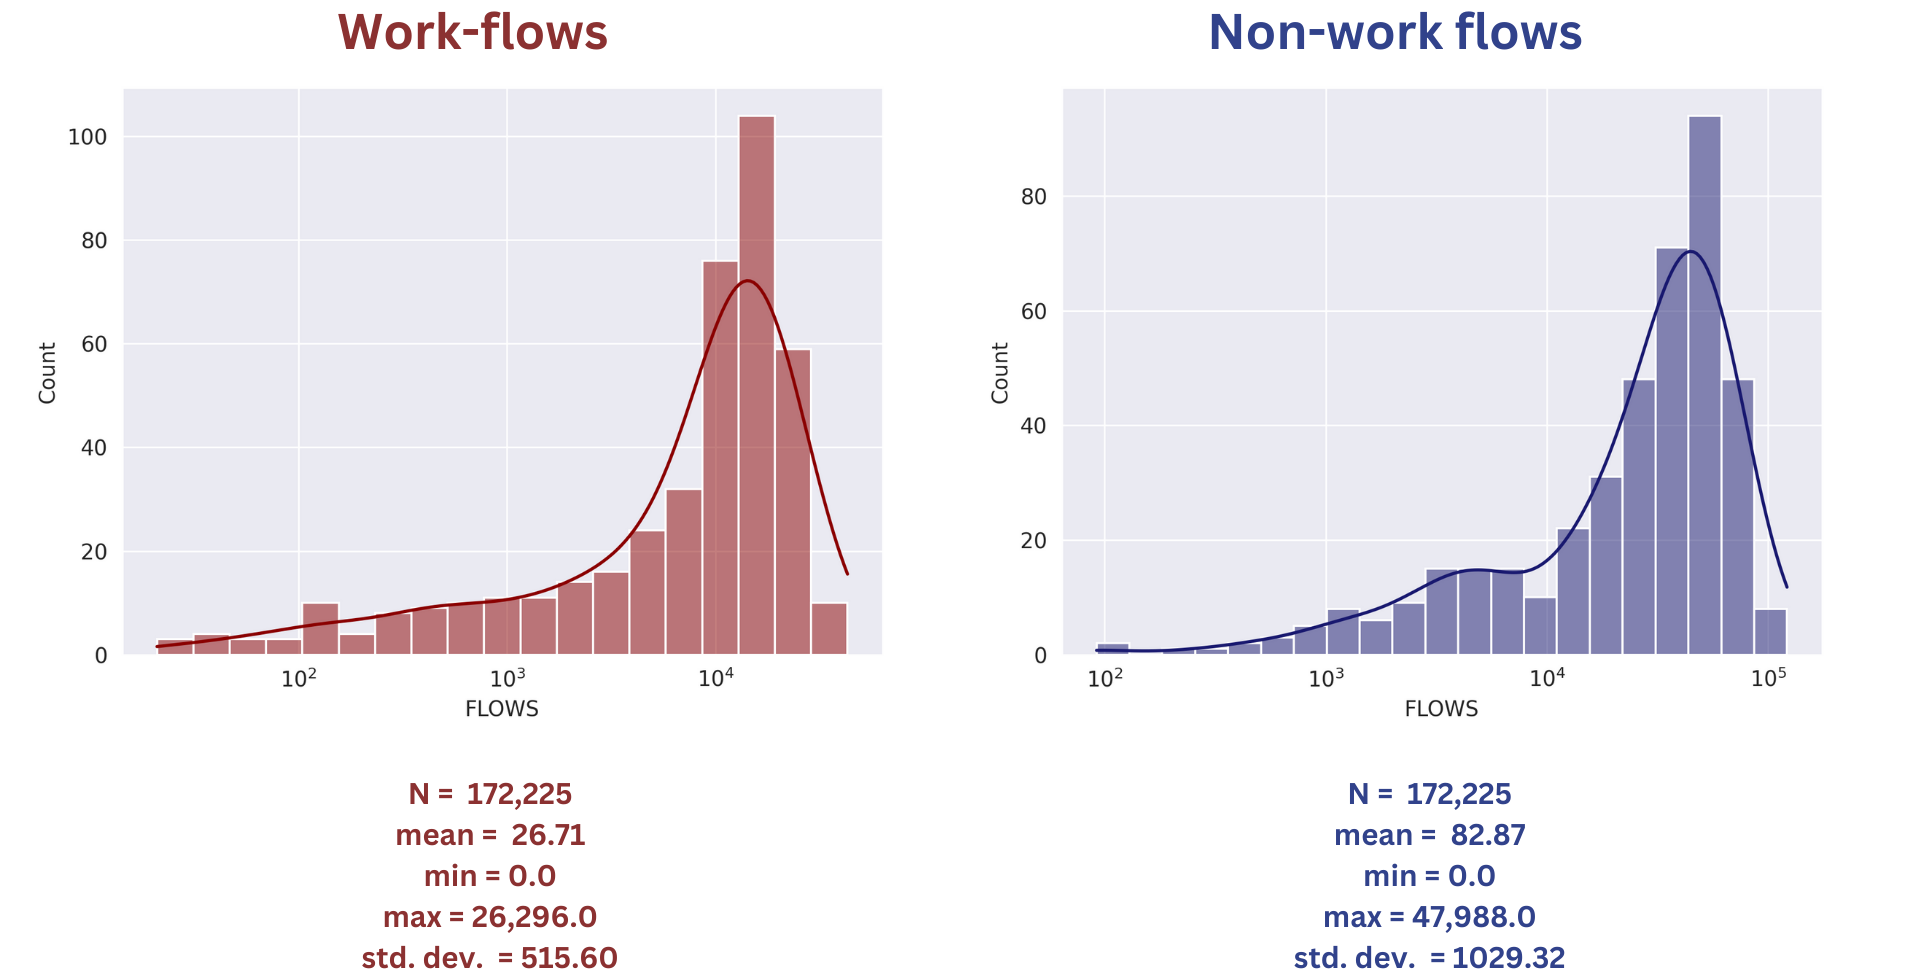
\includegraphics[width=15cm]{Images/Data_values_overview.png}
        \caption{Data Values}
        \label{fig: Data Values Overview}
    \end{figure}

 %%% POINTS OF INTEREST
 
        \subsection{Points of Interest(POI)} 

        The Points of Interest is a dataset categorising various establishments and services across Great Britain, both public and private. The classification system is structured across three levels, each contributing to a comprehensive categorisation of various entities\citep{osPointsInterestClassification2022}.
        
        At the initial level, nine broad Groups serve as the foundation for classification, see Table \ref{table: POIs_groups} . These Groups contain diverse areas such as accommodation, eating and drinking establishments, commercial services, attractions, sports and entertainment facilities, education and health institutions, public infrastructure sites, manufacturing and production facilities, and retail and transport services.

        \begin{table}[H]
\centering
\begin{tabular}{@{}lll@{}}
\toprule
\textbf{COD} & \textbf{Categories} & \textbf{Examples} \\ \midrule
AED & Accommodation, Eating and Drinking & Hotels, Cafes, Pubs \\
CS & Commercial services & Construction, marketing services \\
AT & Attractions & Art Galleries, Zoos, museums  \\
SE & Sport and Entertainment & Sports Complex, Cinemas \\
EH & Education and Health & Health centres, Primary Schools \\
PI & Public infrastructure & Police stations, Wi-Fi hotspots \\
MP & Manufacturing and production &  Conservatories, Farming \\
RT &  Retail & Bakeries, Department stores \\
TR & Transport & Bus stops, Tube stations \\ \bottomrule
\end{tabular}
    \caption{POI categories}
    \label{table: POIs_groups}
\end{table}
        
        Moving to the next level, Level 2, this classification system becomes more refined, consisting of 52 distinct Categories. These Categories further study the entities, providing a more detailed perspective within each Group. Within these categories, specific subcategories define each entity's characteristics. Finally, Level 3 is the most specific classification level, featuring 600 individual Classes. This categorisation ensures a high level of granularity, allowing for precise differentiation and more understanding of the entities within the dataset.

        A hierarchical structure of three distinct levels is evident within this framework\citep{osPointsInterestProduct2022}, as shown in Figure \ref{fig: POI levels}. To provide a concrete example, let us examine the hierarchy within the context of transportation. At the highest level, we have the "Transport" category, a broad umbrella term. Moving down the hierarchy, we encounter the more specific "Category" known as "Bus Transport," which limits the focus to a subset of bus-related transportation. Finally, we reach the most granular level, "Class," exemplified by "Bus Stops". This hierarchical arrangement offers a versatile spectrum of possibilities and classification options, allowing for a comprehensive and structured approach to organising information within the given system.

        \begin{figure}[H]
            \centering
            
\includegraphics[width=12cm]{Images/POI_levels.png}
            \caption{POI levels}
            \label{fig: POI levels}
        \end{figure}


        Due to its increased complexity and adaptability to diverse geographic characteristics, the deep gravity model requires a comprehensive approach when applied to the POI dataset. This model requires a total set of 18 unique geographic features, each contributing specific information about each geographic unit, which, in this context, are represented by hexagons. 
        We derived a classification based on the one in \cite{siminiDeepGravityModel2021} and the one given by the Ordnance Survey, see Table \ref{table: class_POIs}. 

        Therefore, the approach involves considering all available data points for extraction. The categories were restructured because the POI dataset initially included only nine distinct groups, while the Deep Gravity Model required 18 features as input. This restructuring aimed to optimise compatibility with the Deep Gravity Model and provide an equitable information distribution across the new features.


\begin{table}[H]
\centering
\begin{tabular}{@{}ll@{}}
\toprule
\textbf{Item} & \textbf{Category}                             \\ \midrule
1             & Bus Transport                                 \\
2             & Public Transport, Stations and Infrastructure \\
3             & Water                                         \\
4             & Air                                           \\
5             & Education                                     \\
6             & Health                                        \\
7             & Accomodation                                  \\
8             & Restaurants                                   \\
9             & Fast Food                                     \\
10            & Pubs, Bars and Inns                           \\
11            & Cafes, Snack Bars and Tea Rooms               \\
12            & Retail                                        \\
13            & Commercial Services                           \\
14            & Sport and Entertainment                       \\
15            & Attractions                                    \\
16            & Infrastructure and Facilities                 \\
17            & Central and Local Government                  \\
18            & Organisations                                 \\ \bottomrule
\end{tabular}
    \caption{Features classification based on POI dataset}
    \label{table: class_POIs}
\end{table}

        The "Transport" category was disaggregated into four distinct features, each designed to encapsulate the richness of information originally associated with the broader transport aspect. These features effectively retained the essence of the original category names. Moreover, the "Education and Health" group has a similar transformation, grouping many correlated points of interest. Recognising that users often have varying motivations for visiting such locations, this group was split into two separate features: one dedicated to Education and the other to Health.
        
        "Accommodation, Eating, and Drinking" showed many non-work-related opportunities, rendering it one of the most densely populated categories. As a result, this group was divided into four features, reflecting the underlying categories. On the other hand, "Retail," "Commercial Services," and "Attractions" were considered to retain their original classification without further splitting, maintaining a simplified representation. Moreover, the "Public Infrastructure" category garnered significant attention in the regression analysis(Tables \ref{tab:ols-results} and \ref{tab:ols-results-new-bold-color}), categorising it into three distinct features. 
        
        The detailed structure of the feature classification is available in the appendices \ref{appendices1}. It is important to highlight that this new classification strategy does not consider the "level class" despite the limitations in feature count and the analytical complexity. 
    
        Within the Spatial Interaction Model (SIM) framework, the Point of Interest (POI) dataset aggregates the cumulative counts of points relevant to work-related and non-work-related amenities. This categorisation was the foundation for a statistical analysis to unveil the relationships between specific POI groups and Mobility Data Flows. Two separate regression analyses were conducted—one tailored to work-related flows and another to non-work flows.
        
        


 %%% CENSUS DATA
        \subsection{Census data} 
    
    The census data plays a crucial role in both models. In the spatial interaction model, the population is one of the independent variables used to calculate predicted flows alongside factors like distance and attractiveness. Meanwhile, the Deep Gravity Model population data contributes to the location feature vector, which offers a spatial representation for each hexagon. This feature vector includes information from the Points of Interest (POI) dataset and the population size of hexagons obtained from the 2021 census.

    Data consistency is vital, given that the mobility data collected is from 2023, while the Points of Interest data is from 2022. Therefore, including the 2021 census data on London's population becomes crucial for maintaining coherence in the final data analysis. Thus, to prepare the data for use in the models, it was necessary to aggregate it under a common index—specifically, the Mobility data index in Hexagons at level 7. This aggregation step ensures the data is structured consistently for both models' analyses.

    Moreover, population data include an integral part of the 'Population and household estimates for England and Wales: Census 2021'. The Census employs a definition of a usual resident, encompassing individuals who were in the UK on Census Day (21 March 2021) and intended to stay for at least 12 months. Meanwhile, a household is defined as a single person living alone or a collective group.

    \section{Research scope}

%%%%%% DEEP GRAVITY    
        \subsection{Deep gravity Model}


The Deep Gravity model uses various input features to compute the probability $p_{i,j}$ a trip originating at a given location (e.g., $l_i$), to end at any of the $n$ other locations in the region of interest (e.g., $l_j$). The model produces an $n$-dimensional vector of probabilities $p_{i,j}$ for each $j = 1, ..., n$, and this computation is carried out in three steps.
In the first step, input vectors $x(l_i, l_j)$ are created by combining three input features:

\begin{itemize}
        \item $x_i$, representing the feature vector of the origin location $l_i$
        \item $x_j$, representing the feature vector of the destination location $l_j$
\end{itemize}
The geographic distance $r_{i,j}$ between the origin and destination
For each origin location ($l_i$), $n$ input vectors $x(l_i, l_j)$ with $j = 1, ..., n$ are generated, each corresponding to a possible destination within the region of interest.

Next, these input vectors $x(l_i, l_j)$ are fed in parallel into the same feed-forward neural network, consisting of 15 hidden layers. The output of the final layer is a scalar $s(l_i, l_j) \in [-\infty, +\infty]$, referred to as the score, which indicates the likelihood of observing a trip from $l_i$ to $l_j$ according to the model. The probability (i.e., the model's output) is multiplied by the origin's total outflow to determine the generated flow between two locations.

The location feature vector $x_i$ provides a spatial representation of an area and includes features describing properties of the location $l_i$. Its dimension, $d$, corresponds to the total number of considered features.

Additionally, Deep Gravity considers the geographic distance, $r_{i,j}$, between two locations, $l_i$ and $l_j$, measured along the earth's surface between the centroids of the two polygons representing the locations. Each flow in Deep Gravity is described by 39 features, comprising 18 geographic features of the origin and 18 of the destination, along with the distance between the origin and destination and their populations.

    \begin{figure}[H]
        \centering
        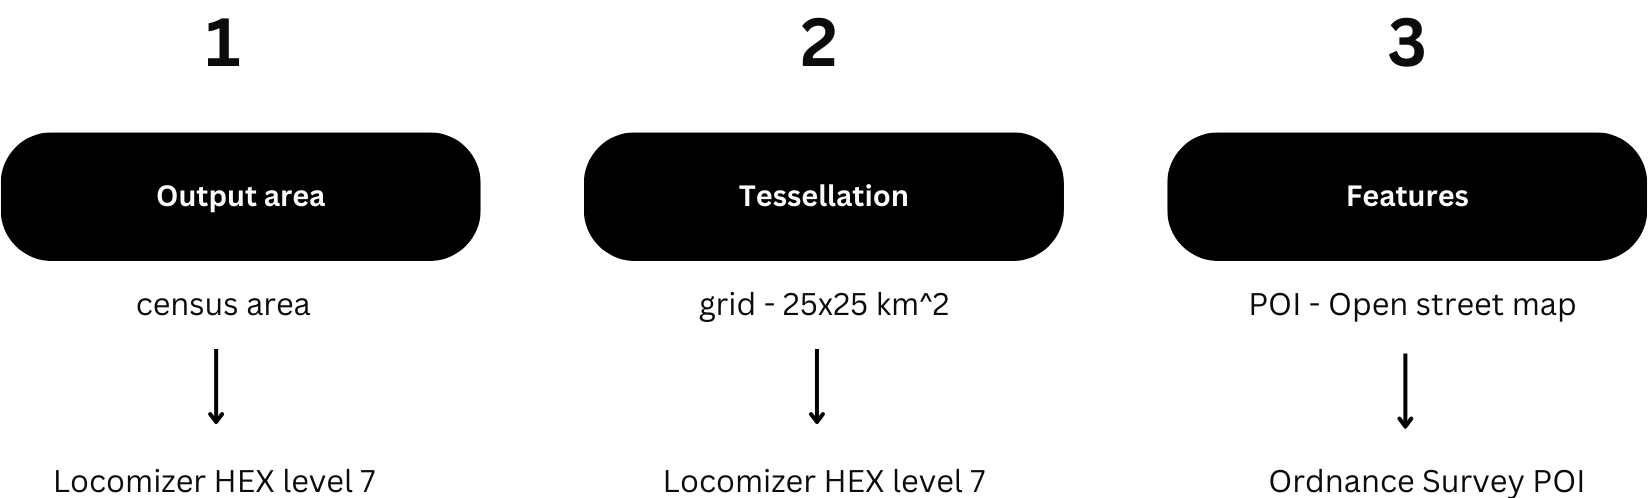
\includegraphics[width=14cm]{Images/DG_Input.png}
        \caption{Deep Gravity Model inputs}
        \label{fig: DG_input}
    \end{figure}

Moreover, deep gravity is a model developed using Pytorch. This Python library conducts real-time execution of dynamic tensor computations, incorporating automatic differentiation and GPU acceleration while maintaining performance levels on par with the fastest contemporary deep learning libraries\citep{paszkePyTorchImperativeStyle2019}.  
    
%%%%%%%%%SPATIAL INTERACTION MODEL

\subsection{Spatial Interaction Model}

The selected spatial interaction model for assessing commuting flows for work and non-work purposes is the production-constrained model, commonly called the retail model. This model offers the advantage of constraining origin information, employing categorical variables, the distance and incorporating data on destination attractiveness. It enables us to gain insights into the dynamics of commute flows from various origins to potential destinations. Our study determined destination attractiveness by considering the total counts of points of interest associated with each flow type, as outlined in the Dataset section.


The availability of the Mobility dataset plays a crucial role, enabling the collection of work and non-work flows between origin and destination hexagons. Consequently, the equation of this model can be expressed as follows:

\begin{equation} \label{eq:1} \tag{1}
T_{ij} = A_i O_i D_j^\gamma d_{ij}^{-\beta}
\end{equation}
where
\begin{equation} \label{eq:3} \tag{2}
A_i = \frac{1}{\sum_j D_j^\gamma d_{ij}^{-\beta}}
\end{equation}

\begin{itemize}
    \item $A_i$ stands for a vector of size $n$ containing the Hexagon origin balancing factors, essential for maintaining the total out-flows in the predicted flows.
    \item $O_i$  represents a vector of size $n$ that indicates the total number of flows originating from the origin $i$ ( Hexagon Origin ID).
    \item $f(d_{ij})=d_{ij}^{-\beta}$  is a function of cost or distance, referred to as the distance-decay function.
\end{itemize}

The model is calibrated using a Poisson Regression function

\begin{equation} \label{eq:4} \tag{4}
\lambda_{ij} = \exp (\alpha_i + \gamma \ln D_j - \beta \ln d_{ij})
\end{equation}
where $\alpha_i$

\begin{figure}[H]
        \centering
        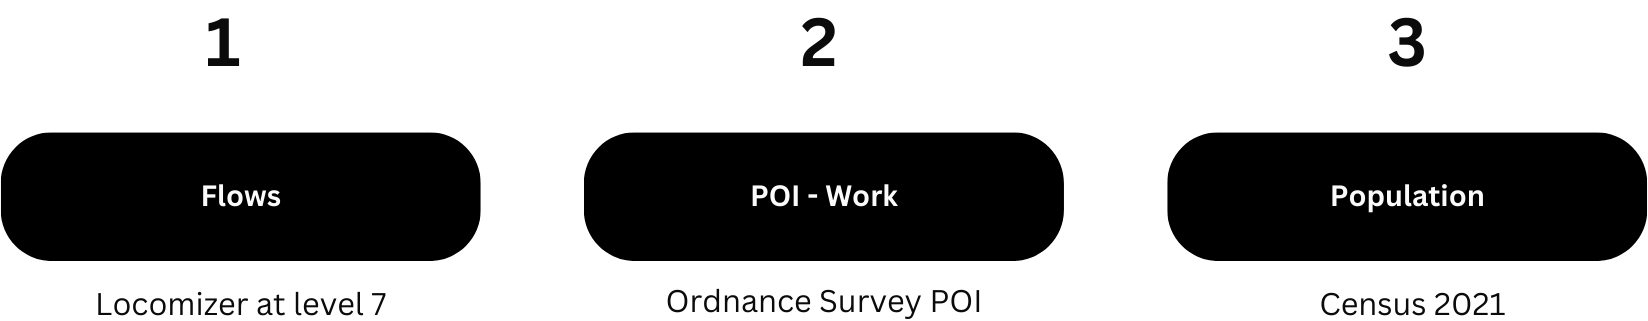
\includegraphics[width=14cm]{Images/SIM_fig.png}
        \caption{Spatial Interaction Model Inputs}
        \label{fig: SIM_input}
    \end{figure}


\subsection{Validation}

The main objective of this study is to use the Root Mean Squared Error (RMSE) to validate models designed for both work and non-work flows. Alongside RMSE, other frequently employed metrics include the Mean Average Error (MAE) and the Mean Average Percentage Error (MAPE). Several error metrics, such as MAE, Mean Squared Error (MSE), RMSE, and MAPE, are frequently employed within this context. These metrics operate within the $[0, \infty ]$ range, where in lower values indicate superior performance. Moreover, The evaluation of flow generation is also carried out by measuring the Common Part of Commuters (CPC) between real and generated flows\citep{lucaSurveyDeepLearning2021}.

As \cite{lucaSurveyDeepLearning2021} stated, MAE considers the absolute value of errors, neglecting the direction of overestimation or underestimation. On the other hand, MSE emphasizes larger errors more significantly than MAE and is also sensitive to outliers. RMSE, the focus of this study, places a greater emphasis on errors than MAE, penalizing models that produce substantial errors. This particular metric is expressed in the same units as the predicted values due to the squared nature of the calculation.

Therefore, this study's pursuit of employing RMSE to validate models dealing with work and non-work flows aligns with established evaluation practices. 

\subsection{Ethical Consideration}

The Locomizer dataset encompasses mobile device-derived information aggregated at hexagons levels, with data updates occurring hourly. The provider of this dataset, LOCOMIZER Ltd, has affirmed its adherence to the General Data Protection Regulation (GDPR) of 2018. This data repository comprises mobility data sourced from mobile devices, procured exclusively with explicit user consent and meticulous observance of local privacy regulations, including but not limited to GDPR.

The dataset adopts a spatial aggregation approach utilizing hexagonal cells, specifically at H3, level 9, and encompasses the geographical expanse of London. Each hexagonal cell corresponds to an approximate area of 0.1 km². The data's temporal granularity follows an hourly structure, which is subsequently summarized daily within the scope of a designated month. Consequently, the intrinsic design of the dataset precludes the identification of individualized locations.

In this context, the Locomizer dataset was obtained by Foster and Partners, the project partner of this dissertation project. This collaborative initiative has established prior authorization for data usage as stipulated within the agreement between the two parties. As a result, the ethical implications surrounding this study were considered low risk, culminating in the project's approval by the Committee for the Centre for Advanced Spatial Analysis (CASA) at University College London (UCL).